%\VignetteIndexEntry{An Introduction to the BPR method}
%\VignetteKeywords{BPR, methylation, gene expression}
%\VignettePackage{BPRMeth}
%\VignetteEngine{knitr::knitr}

\documentclass{article}\usepackage[]{graphicx}\usepackage[usenames,dvipsnames]{color}
%% maxwidth is the original width if it is less than linewidth
%% otherwise use linewidth (to make sure the graphics do not exceed the margin)
\makeatletter
\def\maxwidth{ %
  \ifdim\Gin@nat@width>\linewidth
    \linewidth
  \else
    \Gin@nat@width
  \fi
}
\makeatother

\definecolor{fgcolor}{rgb}{0.345, 0.345, 0.345}
\newcommand{\hlnum}[1]{\textcolor[rgb]{0.686,0.059,0.569}{#1}}%
\newcommand{\hlstr}[1]{\textcolor[rgb]{0.192,0.494,0.8}{#1}}%
\newcommand{\hlcom}[1]{\textcolor[rgb]{0.678,0.584,0.686}{\textit{#1}}}%
\newcommand{\hlopt}[1]{\textcolor[rgb]{0,0,0}{#1}}%
\newcommand{\hlstd}[1]{\textcolor[rgb]{0.345,0.345,0.345}{#1}}%
\newcommand{\hlkwa}[1]{\textcolor[rgb]{0.161,0.373,0.58}{\textbf{#1}}}%
\newcommand{\hlkwb}[1]{\textcolor[rgb]{0.69,0.353,0.396}{#1}}%
\newcommand{\hlkwc}[1]{\textcolor[rgb]{0.333,0.667,0.333}{#1}}%
\newcommand{\hlkwd}[1]{\textcolor[rgb]{0.737,0.353,0.396}{\textbf{#1}}}%

\usepackage{framed}
\makeatletter
\newenvironment{kframe}{%
 \def\at@end@of@kframe{}%
 \ifinner\ifhmode%
  \def\at@end@of@kframe{\end{minipage}}%
  \begin{minipage}{\columnwidth}%
 \fi\fi%
 \def\FrameCommand##1{\hskip\@totalleftmargin \hskip-\fboxsep
 \colorbox{shadecolor}{##1}\hskip-\fboxsep
     % There is no \\@totalrightmargin, so:
     \hskip-\linewidth \hskip-\@totalleftmargin \hskip\columnwidth}%
 \MakeFramed {\advance\hsize-\width
   \@totalleftmargin\z@ \linewidth\hsize
   \@setminipage}}%
 {\par\unskip\endMakeFramed%
 \at@end@of@kframe}
\makeatother

\definecolor{shadecolor}{rgb}{.97, .97, .97}
\definecolor{messagecolor}{rgb}{0, 0, 0}
\definecolor{warningcolor}{rgb}{1, 0, 1}
\definecolor{errorcolor}{rgb}{1, 0, 0}
\newenvironment{knitrout}{}{} % an empty environment to be redefined in TeX

\usepackage{alltt}

\RequirePackage{/usr/local/lib/R/site-library/BiocStyle/resources/tex/Bioconductor}

\AtBeginDocument{\bibliographystyle{/usr/local/lib/R/site-library/BiocStyle/resources/tex/unsrturl}}


\bioctitle[BPRMeth: Methylation features for clustering and prediction]{BPRMeth: Higher order methylation features for clustering and prediction in epigenomics studies}
\author{Chantriolnt-Andreas Kapourani\footnote{C.A.Kapourani@ed.ac.uk}}
\date{Modified: 29 July, 2016. Compiled: \today}
\IfFileExists{upquote.sty}{\usepackage{upquote}}{}
\begin{document}

\maketitle

\tableofcontents

\section{Introduction}
DNA methylation is an intensely studied epigenetic mark, yet its functional role is incompletely understood. Attempts to quantitatively associate average DNA methylation to gene expression yield poor correlations outside of the well-understood methylation-switch at CpG islands.

Here we use probabilistic machine learning to extract higher order features associated with the methylation profile across a defined region. These features quantitate precisely notions of shape of a methylation profile, capturing spatial correlations in DNA methylation across genomic regions.  Using these higher order features across promoter-proximal regions, we are able to construct a powerful machine learning predictor of gene expression, significantly improving upon the predictive power of average DNA methylation levels.

\section{Background}
DNA methylation data produced by High Throughput Sequencing (HTS) technology can be modelled with a Binomial distribution:
\begin{equation}
  m \sim \mathcal{B}inom(t, p)
\end{equation}

In practical studies we are interested in learning the methylation patterns of genomic regions which can be represented by an observation vector $\mathbf{y}$. Let $f(x) = \Phi \big(g(x)\big)$ be a latent function representing the methylation profiles and $g(x)$ be of the form:
\begin{equation}
	 g(x) = \sum\limits_{j=0}^{M-1} w_{j} h_{j}(x)
\end{equation}
where $h_{j}(\cdot)$ can be any basis function, e.g. Radial Basis Function (RBF).

Given $f(x)$ the observations $y_{l}$ for each CpG site are i.i.d. Binomial variables, so we can define the joint log-likelihood in factorised form:
\begin{equation} \label{eq:bpr-likelihood}
 \log p(\mathbf{y} | f) = \sum\limits_{l = 1}^{L} \log \bigg( \mathcal{B}inom\big(m_{l} | t_{l}, \Phi(g(x_{l}))\big) \bigg)
\end{equation}
We refer to this observation model as the Binomial Probit Regression (BPR) likelihood function. \emph{Figure 1} shows the process of learning the methylation profile for a specific promoter region using the BPR model. For a more detailed explanation of the statistical method, see \cite{Kapourani2016}.

\begin{figure}[!ht]
\centerline{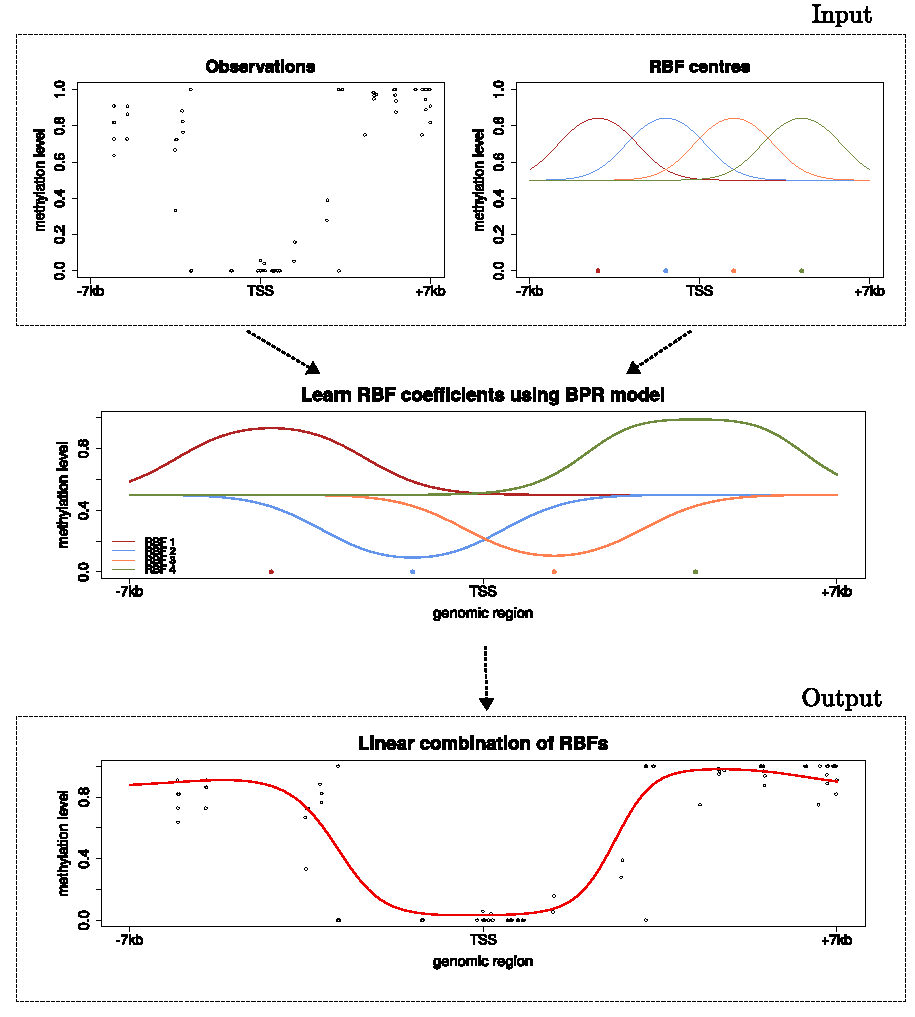
\includegraphics[width=0.70\textwidth]{model-bpr}}
\caption{\small{Illustration of the process for learning methylation profiles using the BPR model. The inputs to the model are the observed methylation levels of the CpGs across the promoter region, plus the number, with their corresponding centres, of the Radial Basis Functions (RBFs), which in this example are chosen to be four. Using this information the BPR model will learn the optimal coefficients for each RBF using maximum likelihood. Finally, we obtain the underlying methylation profile by a linear combination of the fitted RBFs. One should note that the higher the number of RBFs the better the resolution for the methylation profile.}}
\label{fig:model-performance}
\end{figure}

\section{Analysis Pipeline}
\subsection{Sample Data}
In this vignette, as sample data we will use real datasets that are publicly available from the ENCODE project consortium \cite{Dunham2012}. More specifically we will use the K562 immortalized cell line, with GEO: GSE27584 for the RRBS data and GEO: GSE33480 for the RNA-Seq data. We use the preprocessed files, however, we should note that we have converted the RNA-Seq data from \verb|.gtf| to \verb|.bed| format using the \verb|bedops| tool (\href{http://bedops.readthedocs.io} {http://bedops.readthedocs.io}). We keep only the protein coding genes, and for the purposed of this vignette we focus only on \verb|chr12| and \verb|chr13|. Full details of where to download the data and how to preprocess them are included in the Supplementary Material of \cite{Kapourani2016}.

\subsection{Import and read HTS files}
In the \verb|BPRMeth| package we provide methods for reading files generated from HTS experiments with specific formats. Here, we focus on the ENCODE data described above; hence, we will use the wrapper function \Rfunction{process\_haib\_caltech\_wrap} to obtain the final objects for downstream analysis. The user can implement his own methods for different HTS formats and then use the pipeline described in Figure 2 for obtaining the required objects. First, we load the package:
\begin{kframe}
\begin{alltt}
\hlkwd{library}\hlstd{(BPRMeth)}
\end{alltt}
\end{kframe}
and obtain the paths for the RRBS and RNA-Seq files with the following commands:
\begin{kframe}
\begin{alltt}
\hlstd{rrbs_file} \hlkwb{<-} \hlkwd{system.file}\hlstd{(}\hlstr{"extdata"}\hlstd{,} \hlstr{"rrbs.bed"}\hlstd{,} \hlkwc{package} \hlstd{=} \hlstr{"BPRMeth"}\hlstd{)}
\hlstd{rnaseq_file} \hlkwb{<-} \hlkwd{system.file}\hlstd{(}\hlstr{"extdata"}\hlstd{,} \hlstr{"rnaseq.bed"}\hlstd{,} \hlkwc{package} \hlstd{=} \hlstr{"BPRMeth"}\hlstd{)}
\end{alltt}
\end{kframe}

Then, we process both files to obtain the final object which will be used for downstream analysis.  We call the \Rfunction{process\_haib\_caltech\_wrap} function using the default values:
\begin{kframe}
\begin{alltt}
\hlstd{HTS_data} \hlkwb{<-} \hlkwd{process_haib_caltech_wrap}\hlstd{(rrbs_file, rnaseq_file)}
\end{alltt}
\end{kframe}

Among other information, the \verb|HTS_data| object contains the following data that we need for our analysis. First, the promoter methylation data, where only one region is shown below:
\begin{knitrout}
\definecolor{shadecolor}{rgb}{0.969, 0.969, 0.969}\color{fgcolor}\begin{kframe}
\begin{alltt}
\hlkwd{head}\hlstd{(HTS_data}\hlopt{$}\hlstd{methyl_region,} \hlnum{1}\hlstd{)}
\end{alltt}
\begin{verbatim}
## [[1]]
##              [,1] [,2] [,3]
##  [1,] -0.06242857   31    2
##  [2,] -0.06157143   31    0
##  [3,] -0.05985714   31    0
##  [4,] -0.05957143   31    0
##  [5,] -0.04885714    4    0
##  [6,] -0.04557143    4    0
##  [7,] -0.04414286    4    0
##  [8,] -0.03900000    5    0
##  [9,] -0.03857143    5    0
## [10,] -0.03728571    5    0
## [11,] -0.03500000    5    1
## [12,]  0.01171429    7    1
## [13,]  0.01357143    7    0
## [14,]  0.01414286    7    0
## [15,]  0.01457143    7    0
## [16,]  0.02100000    5    1
## [17,]  0.02142857    5    0
## [18,]  0.02285714    5    1
## [19,]  0.02328571    5    1
## [20,]  0.02557143    5    2
## [21,]  0.05871429   61   29
## [22,]  0.06171429   61   30
## [23,]  0.06185714   88   46
## [24,]  0.06200000   61   25
## [25,]  0.06214286   88   50
## [26,]  0.06342857   61   36
## [27,]  0.06357143   88   59
## [28,]  0.06457143   88   59
## [29,]  0.06528571   88   72
\end{verbatim}
\end{kframe}
\end{knitrout}

Each methylation promoter region is an $L_{i} \times 3$ dimensional matrix, where $L_{i}$ denotes the number of CpGs found in region $i$. The columns contain the following information:
\begin{itemize}
\item{ 1st column: Contains locations of CpGs relative to TSS. Note that the actual locations are scaled to the (-1, 1) region. }
\item{ 2nd column: Contains the total reads of each CpG in the corresponding location.}
\item{ 3rd column: Contains the methylated reads each CpG in the corresponding location.}
\end{itemize}

Second, the corresponding log2 transformed gene expression levels for each promoter region, which can be obtained as follows:
\begin{knitrout}
\definecolor{shadecolor}{rgb}{0.969, 0.969, 0.969}\color{fgcolor}\begin{kframe}
\begin{alltt}
\hlkwd{head}\hlstd{(HTS_data}\hlopt{$}\hlstd{gex,} \hlnum{10}\hlstd{)}
\end{alltt}
\begin{verbatim}
##  [1] -3.321928  1.587480  1.792014  2.695450 -2.708765  6.715633  2.109909  1.618953
##  [9] -3.321928 -3.321928
\end{verbatim}
\end{kframe}
\end{knitrout}

Finally, the RNA-Seq data containing annotation data are stored in a \Biocpkg{GRanges} object:
\begin{knitrout}
\definecolor{shadecolor}{rgb}{0.969, 0.969, 0.969}\color{fgcolor}\begin{kframe}
\begin{alltt}
\hlstd{HTS_data}\hlopt{$}\hlstd{rna_data}
\end{alltt}
\begin{verbatim}
## GRanges object with 334 ranges and 3 metadata columns:
##         seqnames                 ranges strand |      ensembl_id   gene_name gene_fpkm
##            <Rle>              <IRanges>  <Rle> |     <character> <character> <numeric>
##     [1]    chr12     [ 569529,  672675]      + | ENSG00000139044    B4GALNT3 0.0000000
##     [2]    chr12     [ 752147,  755044]      + | ENSG00000177406  AC021054.1 2.9052400
##     [3]    chr12     [1021242, 1058888]      - | ENSG00000002016       RAD52 3.3629800
##     [4]    chr12     [1675158, 1703331]      - | ENSG00000171823      FBXL14 6.3775600
##     [5]    chr12     [1901122, 2027870]      - | ENSG00000151062    CACNA2D4 0.0529609
##     ...      ...                    ...    ... .             ...         ...       ...
##   [330]    chr13 [114303172, 114312501]      - | ENSG00000186009       ATP4B   0.00000
##   [331]    chr13 [114321469, 114438724]      + | ENSG00000185974        GRK1   0.00000
##   [332]    chr13 [114462215, 114514926]      + | ENSG00000184497      FAM70B   0.00000
##   [333]    chr13 [114523523, 114567046]      - | ENSG00000183087        GAS6   8.55437
##   [334]    chr13 [114747193, 114898095]      - | ENSG00000185989       RASA3  15.20510
##   -------
##   seqinfo: 2 sequences from an unspecified genome; no seqlengths
\end{verbatim}
\end{kframe}
\end{knitrout}

\bibliography{BPRMeth_vignette}

\end{document}
